% !TeX root = ../main.tex

\chapter{討論}

針對兩種平坦隱沒模型,各有不同的觀測資料特徵。
本章將模型結果與觀測資料進行比對,討論兩種平坦隱沒類型所具有的構造特色與岩漿作用狀態。
最後,對於不同類型的平坦隱沒形成原因,將兩種模型分開討論。

除此之外,祕魯平坦隱沒區域的地震能量是周遭隱沒帶的3-5倍,表示在平坦隱沒下,隱沒板塊與上覆板塊高度耦合(coupling),摩擦力極大(\citealp{Gutscher2000A})。

\section{隱沒系統的熱構造與耦合關係}
隱沒板塊的耦合概念在1970年代晚期開始盛行(\citealp{uyeda1979back}; \citealp{ruff1980seismicity}),\citealp{uyeda1979back}以隱沒板塊的年紀將隱沒帶分成兩種類型:第一種是年輕隱沒板塊的智利型(Chilean type)隱沒帶,第二種是年老隱沒板塊的馬尼亞納型(Mariana type)隱沒帶,示意圖如圖\ref{fig::end-member subduction}所示。
\begin{figure*}[htp]
    \centering
    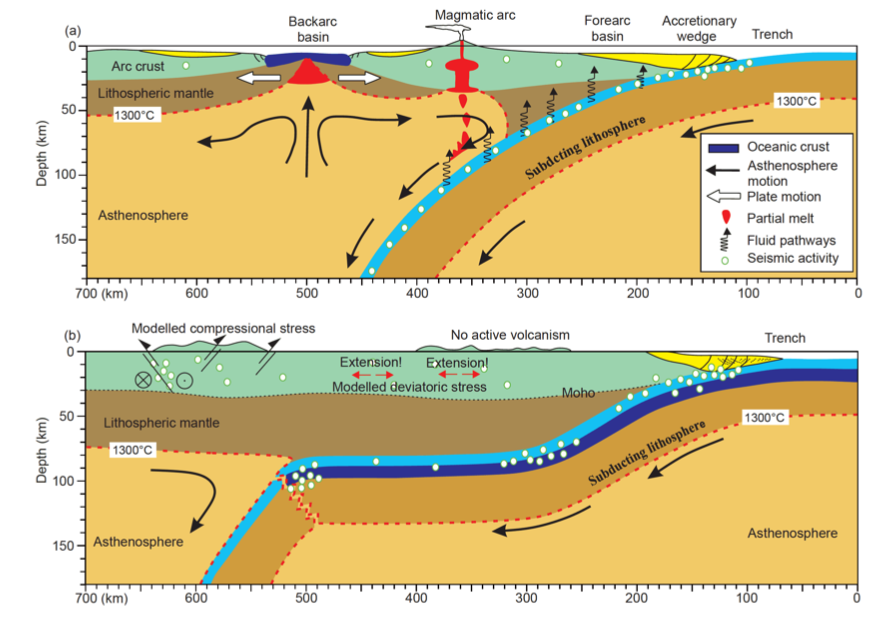
\includegraphics[width=6in]{2020subduction_type.png}
    \caption[隱沒帶的兩種型態示意圖]{隱沒帶的兩種型態示意圖,摘自\citealp{Yan2020}。}
    \label{fig::end-member subduction}
\end{figure*}

智利型隱沒帶因隱沒板塊溫度較高、密度較小,故隱沒傾角較低,在聚合板塊交界處產生較大的板塊接觸面積,可見圖\ref{fig::end-member subduction}b。
通常此類隱沒帶會容易產生低角度的班尼奧夫帶,地震事件特徵以逆衝斷層為主,且發生過多起大規模(Mw>8.0)地震事件。
上覆板塊側有顯著的壓縮應力,可能會在弧後出現許多皺褶與斷層,因此智利型隱沒帶亦會被視為強耦合(strong coupling)隱沒帶。
反之馬尼亞納型隱沒帶中隱沒板塊年紀較大、密度較大,重力較大造成隱沒板塊垂直分量上的拉力較大、隱沒傾角較高,與上覆板塊的接觸面積相對較小,可見圖\ref{fig::end-member subduction}a。
此類隱沒帶的應力不易累積,容易發生潛移活動,地震事件規模較小且通常為伸張地震,故馬尼亞納型隱沒帶又可稱為弱耦合(weak coupling)隱沒帶。
此外,高角度的隱沒板塊造成地函楔容易發生強烈對流,伴隨隱沒帶的部分熔融作用,在上覆板塊側發生拉張現象,可能會產生弧後張裂(back-arc spreading)。

過去的研究注意到智利上覆板塊的地殼地震事件數目在平坦隱沒區域較多(\citealp{jordan1983andean}; \citealp{smalley1993basement}),表明平坦隱沒區域具有比正常隱沒帶更強的板塊間耦合。
\citealp{gutscher2002andean}統計智利沿岸在距海溝250-800公里的所有地震事件所釋放之能量總和,以南北向一度以內為單位,獲得板塊釋放的地震能量直方圖。
總體而言,智利中部平坦隱沒上方的板塊所釋放出的地震能量比北部玻利維亞段高出5倍,比南段智利高出10倍。
\citealp{jordan1983andean}分析智利沿岸大地震的震源機制解,顯示該區域以壓縮型地震主導,P軸垂直於海溝,他認為隱沒邊界應力有效傳遞到上覆板塊,並且在平坦隱沒段有更高程度的板塊間耦合。

\begin{figure*}[htp]
    \centering
    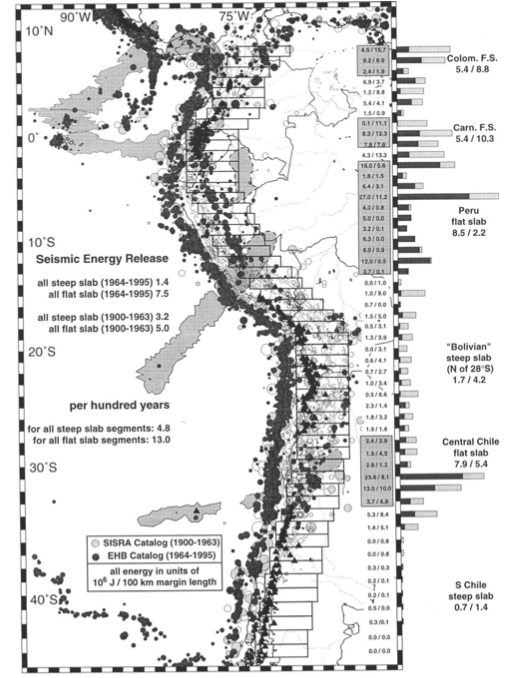
\includegraphics[width=4in]{Seismicity and Energy of Andes.png}
    \caption[智利沿岸自21$^\circ$S到44$^\circ$S的上板塊地震活動統計分析]{智利沿岸自20$^\circ$S到40$^\circ$S的上板塊地震活動統計分析,摘自\citealp{gutscher2002andean}。這裡採用深度<70公里的地震事件總能量,單位為10$^6$焦耳。右側數字表示1900-1963年/1964-1995年間所示分的第鎮能量。數字下灰色底框標示出平坦隱沒段的位置。
    }
    \label{fig::Chile_seismicity}
\end{figure*}

本研究智利參考模型的水平應力(Sxx)剖面圖如圖\ref{fig::Sxx_and_Pressure_Chile}a所示。
上覆板塊側的水平應力在平坦隱沒段上地殼處有較小值,表示壓縮應力的存在。
上覆板塊的壓縮應力在水平方向上可分為兩區域,第一個區域位在絕對座標550-650公里之間,其下方對應到隱沒板塊上凹變形處位置。
第二個區域位於絕對座標750-800公里,對應到隱沒板塊下傾位置。
該結果表示模型中隱沒板塊的應力可以傳遞至上覆板塊,並且對上覆板塊的水平壓縮應力有顯著影響。
除此之外,動水壓力剖面同樣可以觀察到類似的現象,在圖\ref{fig::Sxx_and_Pressure_Chile}b中,上覆板塊淺層於絕對座標550-650公里處有很大的正壓力,與圖\ref{fig::Sxx_and_Pressure_Chile}a中的壓縮應力位置相似,同為平坦隱沒板塊所造成的應力貢獻。


\begin{figure*}[h]
    \centering
    \includegraphics[width=5in]{Sxx_and_Pressure_Chile_of_150_v1.pdf}
    \caption[參考模型中於30 Myr的動水壓力剖面]{參考模型中於30 Myr的動水壓力剖面。}
    \label{fig::Sxx_and_Pressure_Chile}
\end{figure*}

儘管如此,墨西哥平坦隱沒並沒有強耦合的特徵。
\citealp{PerezCampos2008}的接收函數結果顯示墨西哥的隱沒板塊平坦段深度直接位於莫合面下方,因此隱沒板塊與上覆板塊的接觸面材質為海洋地殼與下部大陸地殼的成分,幾乎不包含任何大陸地函軟流圈(continental mantle asthenosphere),此時板塊介面在聚合過程中理論上應產生很大的摩擦力。
此外,墨西哥隱沒帶被視為侵蝕型隱沒(subduction erosion)(\citealp{stern2011subduction}),其證據包含現今外海的沉積物厚度約200公尺(\citealp{manea2003sediment}),並且擁有快速的聚合速率(\citealp{o2005uncertainties})。
再配合年輕隱沒帶的低傾角隱沒特徵,墨西哥平坦段聚合板塊接觸面積極大。
種種物理跡象表明該區域應該為強耦合環境。
然而墨西哥平坦隱沒段的地震活動度極低,格雷羅無震帶(Guerrero gap)(\citealp{kostoglodov2003large})便位於平坦段上,表明平坦段並非處於強耦合狀態。
除此之外,平坦隱沒上方並沒有顯著的水平壓縮現象(\citealp{nieto2006latest}; \citealp{moran2007cenozoic},這與強耦合的特徵互相矛盾。
對此,\citealp{Manea2011Thermal}模擬墨西哥平坦隱沒剖面的熱構造。
海洋地殼與沉積物決大部分在距海溝250公里前便完成脫水,大量的水分可能釋放進入下大陸地殼中,導致岩石強度降低,不容易累積大量應力。
該地區的非火山微震(non volcanic tremor)發生位置與海洋地殼的脫水位置相吻合\citealp{Manea2011Thermal},慢地震(slow slip event)事件位置則與沈積物的脫水位置吻合\citealp{Song2009}。
大量的微震與慢地震事件暗示著該區域為弱耦合隱沒帶。

本研究墨西哥參考模型的水平應力(Sxx)剖面圖如圖\ref{fig::Sxx_and_Pressure_Mexico}a所示。
上覆板塊側的水平應力在上部地殼與下部地殼底部各有一層高區。
此外,在絕對座標700公里與800公里處的火山島弧下方也具有地區性的水平應力小值,其為火山形成的荷重所造成。
與智利參考模型相比,墨西哥參考模型的上覆版塊沒有顯著的壓縮應力存在。
動水壓力剖面同樣可以觀察到類似的現象,如圖\ref{fig::Sxx_and_Pressure_Mexico}b所示,上覆板塊側除了上下地殼交界處與莫合面處有較高的正壓力外,並沒有顯著來自隱沒板塊介面所提供的正壓力。
\begin{figure*}[h]
    \centering
    \includegraphics[width=5in]{Sxx_and_Pressure_Mexico_of_150_v1.pdf}
    \caption[參考模型中於30 Myr的水平應力剖面]{參考模型中於30 Myr的水平應力剖面。}
    \label{fig::Sxx_and_Pressure_Mexico}
\end{figure*}

本研究於第\ref{墨西哥隱沒帶地球物理觀測}節與第\ref{墨西哥參考模型結果}節皆有提及地震學研究在墨西哥平坦隱沒區域的板塊介面中發現一層低速層(\citealp{PerezCampos2008}),\citealp{Song2009}估計該低速層厚度約3-5公里且剪力波(V$_S$)速度約每秒2-2.7公里,速度大約降低26-40$\%$。
過去對於該低速層的成分有諸多解釋,\citealp{Song2012SC}認為其為經歷強烈剪切的變質岩成分。
\citealp{Manea2017}則認為該弱耦合物質為殘餘的蛇紋岩。

\begin{figure*}[h]
    \centering
    \includegraphics[width=5in]{Phase_compare_of_150_v1.pdf}
    \caption[參考模型中於30 Myr的岩相剖面]{參考模型中於30 Myr的岩相剖面。}
    \label{fig::phase_compare}
\end{figure*}

從墨西哥參考模型的岩相圖\ref{fig::phase_compare}可見隱沒板塊與大陸地殼的介面中具有厚度4-8公里、以沉積岩為主參雜少許蛇紋岩化橄欖岩的弱物質。
由於該弱物質層的岩石強度極弱,故隱沒板塊介面成為弱耦合介面,上覆板塊的壓縮應力較小。

因此,並非所有低傾角隱沒帶皆具有強耦合的特徵。

\section{平坦隱沒中的埃達克岩}\label{平坦隱沒中的埃達克岩}
埃達克岩(Adakite)最初由\citealp{kay1978aleutian}觀測阿留申群島中Adak Island上一種高La/Yb、高Sr/Y以及富含大離子半徑元素(large ion lithophile (LIL)- element-rich)的安山岩,其特徵與一般的火山島弧安山岩不相同,爾後\citealp{defant1990derivation}將其命名為埃達克岩(adakite)。
通常一般火成岩研究利用Sr/Y-Y作圖與(La/Yb)$_N$-Yb$_N$作圖區別埃達克岩與一般的島弧中酸性安山岩,如圖\ref{fig::AdakiteY}。

\begin{figure*}[h]
    \centering
    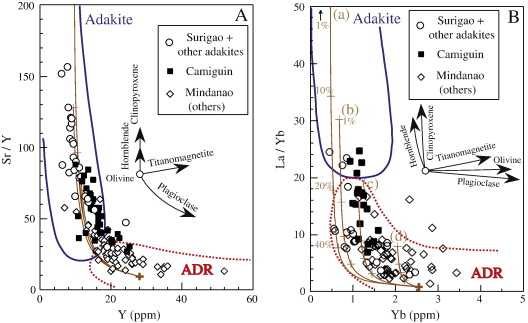
\includegraphics[width=6in]{AdakiteY.jpg}
    \caption[Sr/Y-Y作圖與(La/Yb)$_N$-Yb$_N$作圖]{(A)Sr/Y-Y作圖與(B)(La/Yb)$_N$-Yb$_N$作圖,摘自\citealp{castillo2012adakite}。通常用於區分埃達克岩與普通島弧安山岩、石英岩與流紋岩(normal arc andesite, dacite and rhyolite, ADR)。紫色實線邊界來自於\citealp{richards2007special}所提出菲律賓中南部埃達克岩與普通島弧安山岩的資料。}
    \label{fig::AdakiteY}
\end{figure*}

埃達克岩反映岩漿源環境來自高壓變質基性岩,過去認為埃達克岩是年輕的(< 25 Ma)隱沒海洋玄武岩發生部分熔融產生的中酸性火山岩(\citealp{defant1990derivation}),不過因為埃達克岩的定義來自岩石中化學組成分定量分析,因此埃達克岩性質的火成岩可能由多種不同機制而產生(\citealp{martin2005overview}),以下列出最常見的四種:

(1)隱沒海洋地殼加上海洋沉積物的熔融(\citealp{defant1990derivation}),具有低Nd、高Sr同位素特徵(\citealp{gomez2003temporal})。

(2)增厚大陸下地殼底部的基性岩熔融。
在高壓環境下,基性岩密度過高時無分穩定存在於大陸地殼底部,因此部分熔融產生。
比較可能會發生在島弧岩漿作用事件中末期,需要長時間的地殼增厚(\citealp{kay2002magmatism})。

(3)普通島弧安山岩混合地殼岩漿,其稱為low-SiO$_2$ adakite (\citealp{martin2005overview})。

(4)部分具有埃達克岩特徵的火成岩源區來自一般的島弧基性岩漿,在高壓(> 12 kbar)環境下,石榴子石結晶分化下的產物(\citealp{moyen2009high})。

如今埃達克岩雖然有化學分析上的明確定義,然而其構造意義趨向發散。
一般來說,上述成因中,只有(1)與(2)兩種成因可被稱為埃達克岩,而(3)與(4)所產生之高Sr/Y類似因物質交換而繼承埃達克岩特徵,稱作類埃達克岩(Adakite-like rocks)(\citealp{kay2002magmatism}; \citealp{goss2013andean})。

早期在南美洲的平坦隱沒區域發現部分埃達克岩的紀錄,\citealp{Gutscher2000Bcan}為此提出一概念模型,為平坦隱沒特殊的溫壓條件所生成埃達克岩。

平坦隱沒具有與正常隱沒帶不同的溫壓路徑,由於其地殼在等深度下維持不變長達近80公里,在整段平坦段中壓力不變,但越靠內陸側之岩石溫度越高,此時鐵鎂岩相與沉積岩相很有可能會通過固熔點,導致海洋地殼發生部分熔融。


埃達克岩的特徵之一為高Gd/Yb與高SiO$_2$,如圖\ref{fig::Cocos_geochemisty}b與圖\ref{fig::Cocos_geochemisty}c所示。

這個趨勢在15 Ma左右被侵入的埃達克岩中斷(\citealp{mori2007effects}),見圖\ref{fig::Cocos_geochemisty}a紅色與藍色點,值得注意的是,具有埃達克岩特徵的樣本幾乎都與海溝距離超過400公里。

目前學界一致認同墨西哥平坦隱沒區域所發現的埃達克岩樣本皆為隱沒海洋地殼與沉積物的產物(\citealp{Gutscher2000Bcan}; \citealp{ferrari2012dynamic}; \citealp{Manea2017})。

\begin{figure*}[ht!]
    \centering
    \includegraphics[width=6in]{Cocos_Volcano.pdf}
    \caption[墨西哥區域火山島弧地球化學分析,摘自\citealp{ferrari2012dynamic}]{
    }
    \label{fig::Cocos_geochemisty}
\end{figure*}



目前提出兩種概念模型解釋智利區域的埃達克岩形成原因,
(1)火成岩岩漿源由於大陸地殼底部增厚,導致最底部的地殼在石榴子石穩定場下發生部分熔融。
或者岩漿源可能是部分熔融與下大陸地殼物質的混合物。
(2)隱沒侵蝕將弧前陸塊岩石帶入地函中,導致部分地函源岩漿與弧前陸塊混合形成埃達克岩岩漿庫。
安地斯區域的埃達克岩難以用第一種模型解釋之,因岩漿作用發生在早至晚中新世(Early to Late Miocene, 23 Ma-9 Ma),難以解釋地殼在該短時間段之內發生顯著增厚現象(\citealp{kay2002magmatism})。
\citealp{kay2002magmatism}所提出的概念模型如圖\ref{fig::Nazca_geochemisty}。

\begin{figure*}[h!]
    \centering
    \includegraphics[width=6in]{Nazca_magmatism_concept.png}
    \caption[智利平坦隱沒區域岩漿活動概念模型]{智利平坦隱沒區域岩漿活動概念模型,摘自\citealp{kay2002magmatism}
    }
    \label{fig::Nazca_geochemisty}
\end{figure*}

\section{為什麼會形成平坦隱沒}
由於平坦隱沒的形成原因至今依然是一開放性問題,以下將討論隱沒帶中不同構造區對隱沒系統的影響,以及本研究模型中產生平坦隱沒的可能關鍵原因。
最後會討論可能影響隱沒傾角的原因。
\subsection{均質的隱沒板塊}
本研究的兩種參考模型中,隱沒板塊上皆不存在任何非均質(heterogeneous)構造或任何例外的物理行為。
同\ref{平坦隱沒的數值模型}所述,過去的數值模型提出許多降低隱沒系統重力力矩的可能原因,包含加入一段不會發生玄武岩相變的海洋地殼(\citealp{Liu2016}; \citealp{Gerya2009})、延後榴輝岩相的相變時間(\citealp{van2002role})、增厚隱沒海洋地殼(\citealp{Liu2016}; \citealp{axen2018basal})、降低整體隱沒岩石圈密度(\citealp{Gerya2009})以及設計隱沒板塊隱沒後斷裂(\citealp{Liu2016}; \citealp{axen2018basal})等。

早期研究認為隱沒的海洋高原最有可能是平坦隱沒的形成原因(\citealp{gutscher2002andean}),此概念甚至被寫進書籍裡。
\citealp{Skinner2013}利用磁力條帶重建納茲卡板塊上海洋高原及洋脊位置,並且計算其隱沒進入南美板塊的時間。
他們的研究表明隱沒的地殼增厚體與平坦隱沒發生時間錯開,因此平坦隱沒的形成原因可能無法完美的被地殼增厚體所解釋。
\citealp{Marot2014}利用表面波地震層析成像探討智利平坦隱沒下方的速度構造,他的結果沒有看到任何異常的隱沒地殼,並支持納茲卡板塊在速度上與厚度上皆是均勻的構造。
放眼至地球上其他區域,許多區域皆有海脊隱沒的證據,例如勘察加半島(Kamchatka)有皇帝海脊(Emperor Ridge)隱沒、琉球(Ryukyu)有大東海脊(Daito Ridge)隱沒以及馬里亞納(Mariana)與馬庫斯—內克海脊(Marcus-Necker Ridge)隱沒,然而只有秘魯與智利有平坦隱沒的特徵。
另一個問題是,在墨西哥有平坦隱沒的特徵,然而墨西哥沒有任何海脊或海洋高原的隱沒紀錄,因此增厚的海洋地殼發生平坦隱沒的理論近年來逐漸站不住腳(\citealp{schellart2020control}; \citealp{Schellart2021})。

% 由於上述的前人研究並沒有討論到墨西哥區域的平坦隱沒,這裡僅先以智利參考模型的結果做討論。
% 參考模型中,隱沒板塊地殼在50個百萬年內皆維持7公里,並且整段隱沒板塊維持連續。
% 本研究嘗試隱沒增厚的海洋地殼,然而並沒有看到顯著的浮力增加現象。


\subsection{上覆板塊}
\subsubsection{上覆板塊的溫度構造}
由於本研究的兩種參考模型使用不同的溫度構造,所以以下將會分為兩個部分做說明。

\citealp{Thermal2012}的數值模型討論上覆板塊的溫度構造與平坦隱沒的關係,他們結果顯示較冷硬的上覆板塊較容易產生低傾角的隱沒帶。
他們的模型中,上覆板塊與隱沒板塊皆使用平板冷卻模型(plate cooling model),固定板塊底部的溫度為攝氏1450$^\circ$且板塊厚度為95公里。
但該結果與本研究的結果互相矛盾。

在智利參考模型中,由於智利地區的溫度構造研究並沒有太多過去前人約束,因此,本研究對上覆板塊厚度做一系列測試,討論上覆板塊溫度構造對隱沒板塊構造的影響。
上覆板塊厚度測試範圍為120公里、130公里、140公里、150公里與160公里,在智利參考模型中,板塊的溫度構造由攝氏10$^\circ$的地表線性遞增至板塊底部為攝氏1330$^\circ$,因此,測試的五個模型具有不同的地溫梯度。
每個模型的隱沒傾角隨時間變化如圖\ref{fig::compare_dip_thermal},其中,隱沒傾角的計算方式如圖\ref{fig::dip_of_slab}所示,隱沒板塊自海溝到深度150公里之間的直線與水平之夾角$\alpha$。

\begin{figure*}[h]
    \centering
    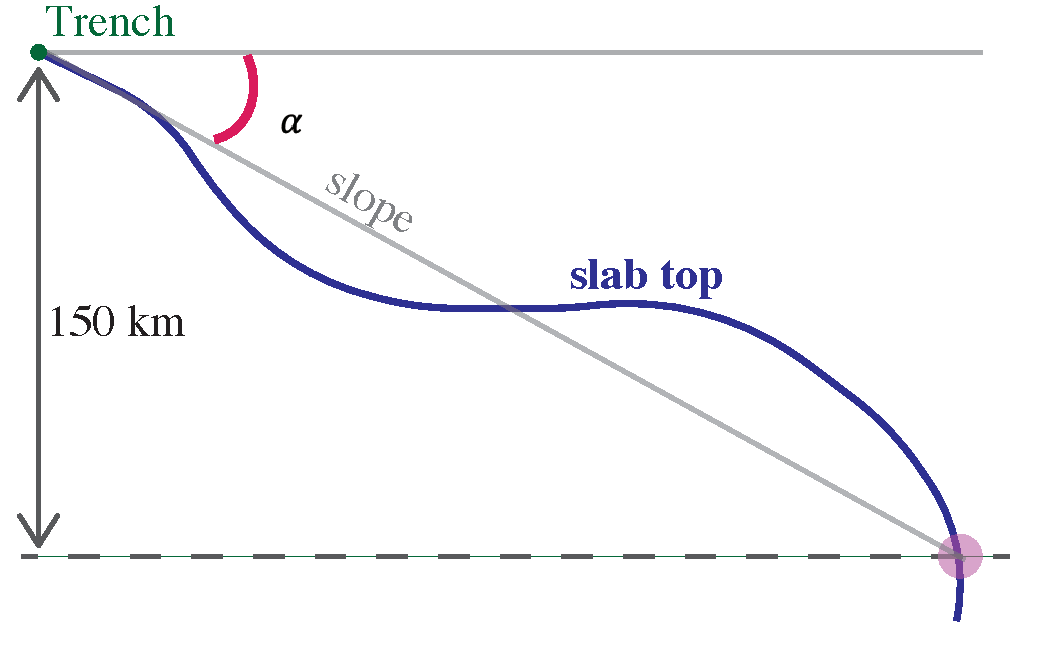
\includegraphics[width=4in]{dip_of_slab.pdf}
    \caption[本研究中隱沒傾角的計算方式]{本研究中隱沒傾角的計算方式。}
    \label{fig::dip_of_slab}
\end{figure*}

\begin{figure*}[h]
    \centering
    \includegraphics[width=5in]{compare_dip_Nazca_a0701_Nazca_a0705_v1.pdf}
    \caption[不同上覆板塊厚度模型之隱沒傾角隨時間變化]{不同上覆板塊厚度模型之隱沒傾角隨時間變化。}
    \label{fig::compare_dip_thermal}
\end{figure*}

該結果表明,上覆板塊厚度在140公里以內的隱沒傾角在模型時間20個百萬年後可低於15$^\circ$以內,反之,上覆板塊厚度150公里與160公里的模型隱沒傾角在任何時間上都高於25$^\circ$。
若將每個模型的隱沒板塊頂部隨深度繪出,可獲得圖\ref{fig::compare_geometry}。
從圖中可見,平坦隱沒特徵僅出現在上覆板塊厚度為120公里、130公里、140公里的三個模型中,而上覆板塊厚度150公里與160公里的兩個模型則是一個正常傾角的隱沒帶。
這意味著上覆板塊的溫度構造會大程度的影響隱沒板塊的隱沒構造,並且,高溫的環境較容易生成平坦隱沒。
該結果與\citealp{Thermal2012}的結果相反。
此外,圖\ref{fig::compare_geometry}顯示平坦隱沒的平坦長度與深度在不同模型中有出入,藉由計算模型中平坦段的長度與深度,可獲得圖\ref{fig::compare_slab_time}
\begin{figure*}[h]
    \centering
    \includegraphics[width=5in]{multi_slab_analysis_Nazca_a0701_Nazca_a0705_v1.pdf}
    \caption[不同上覆板塊厚度模型在50個百萬年的隱沒板塊構造]{不同上覆板塊厚度模型在50個百萬年時隱沒板塊於150公里以上之構造,幾何形狀取自隱沒板塊頂部,使用5公里移動平均平滑離散化的網格。}
    \label{fig::compare_geometry}
\end{figure*}

較高溫的上覆板塊構造會在較淺的深度形成較長的平坦隱沒段,與\ref{智利參考模型結果}的推測相同,平坦段深度大致與原先大陸岩石圈攝氏 800$^\circ$ 等溫線深度相同,因此較薄的大陸岩石圈有較淺的平坦隱沒段。
\begin{figure*}[h]
    \centering
    \includegraphics[width=5in]{Nazca_a0701_Ref_Nazca_flatslab_length.pdf}
    \caption[不同上覆板塊厚度模型的平坦段長度與深度]{不同上覆板塊厚度模型的平坦段(a)長度與(b)深度。}
    \label{fig::compare_slab_time}
\end{figure*}

三個模型的平坦隱沒段長度差亦可達超過100公里。

在墨西哥區域,\citealp{Manea2011Curie}曾經利用地磁資料計算墨西哥南部的居禮溫度(Curie temperature)面深度,進而獲得隱沒帶區域的溫度構造觀測資料。
在他們的研究中,針對兩條垂直於海溝的剖面進行討論,一條剖面為平坦隱沒段,另一條剖面為正常隱沒段。
平坦隱沒剖面在弧後區域具有較淺的居禮溫度面,由地磁獲得的估計居禮溫度面在弧後區深度約20-25公里,由他們研究中的熱模型推得的居禮溫度面深度約30公里左右,本研究墨西哥參考模型初始穩定大陸的居禮溫度面深度為28.5公里。
正常隱沒剖面的居禮溫度面範圍較大,地磁資料的結果由15-30公里不等,然而他們的熱模型結果表示居禮溫度面在弧後區約落在42公里左右。
\begin{figure*}[h]
    \centering
    \includegraphics[width=5in]{CurieMexico.png}
    \caption[墨西哥兩條剖面的居禮溫度面與熱構造模型]{墨西哥兩條剖面的居禮溫度面與熱構造模型,摘自\citealp{Manea2011Curie}}
    \label{fig::CurieMexico}
\end{figure*}

為了測試該熱模型結果是否與本研究吻合,因此,將墨西哥參考模型的地溫梯度從原先40公里以前的每公里攝氏20$^\circ$改為每公里15$^\circ$,此時初始模型的居禮溫度面約為38公里。
\begin{figure*}[h]
    \centering
    \includegraphics[width=5in]{Curie_Point_v1.pdf}
    \caption[不同地溫梯度的墨西哥模型在30個百萬年的隱沒板塊構造與580$^\circ$等溫線]{不同地溫梯度的墨西哥模型在30個百萬年的隱沒板塊構造(黑線)於150公里以上之構造與580$^\circ$等溫線(紫線),幾何形狀取自隱沒板塊頂部,使用5公里移動平均平滑離散化的網格。}
    \label{fig::Curie_Point_model}
\end{figure*}

圖\ref{fig::Curie_Point_model}顯示與\citealp{Manea2011Curie}類似的居禮溫度面結果,並且,與智利參考模型的結論相似,較高溫的大陸岩石圈較容易產生平坦隱沒。
兩模型的吸力力矩隨時間變化之結果如圖\ref{fig::thermal_Cocos_suction},
\begin{figure*}[h]
    \centering
    \includegraphics[width=5in]{thermal_Cocos_suction.pdf}
    \caption[不同地溫梯度的墨西哥模型之吸力力矩。]{}
    \label{fig::thermal_Cocos_suction}
\end{figure*}

\subsubsection{上覆板塊的強度}


\subsection{地函楔中的動水壓力矩}
\citealp{Manea2017}與\citealp{Yan2020}提及隱沒帶脫水作用應是對動水壓力力矩有重大影響的因素之一。
大量的脫水會降低地函楔黏滯度與地函岩石強度,因此可能會降低地函動水壓力力矩的量值。
除了脫水作用外,岩漿作用也是另一個會影響地函楔黏滯度與岩石強度的因素。
在模型中,當地函楔發生部分熔融後,岩漿庫所產生的潛熱造成地函楔局部溫度增加,進而降低地函楔的黏滯度。
過去的數值模型鮮少討論岩漿作用對隱沒系統的動水壓力矩影響,因此本研究對岩漿參數做一系列測試,用以探討兩者的關聯。
本節會先利用蛇紋岩厚度測試脫水作用對動水壓力矩的影響,再討論岩漿作用與動水壓力矩的關係,由於本研究中,智利參考模型的平坦隱沒上方包含地函楔,因此本節僅會測試與討論智利參考模型。
\subsubsection{隱沒帶的脫水作用}
由於本研究中,數值模型的蛇紋岩產生量可自由控制,因此測試不同蛇紋岩厚度對智利參考模型的影響。
受限於網格解析度,因此測試厚度為3公里、6公里、9公里、12公里、18公里與30公里。
不同蛇紋岩厚度的模型的隱沒傾角隨時間變化如圖\ref{fig::compare_dip_thermal},隱沒板塊自海溝到深度150公里之間的直線與水平之夾角$\alpha$。

\begin{figure*}[h]
    \centering
    \includegraphics[width=5in]{compare_dip_serpentinite_thickness_Nazca.pdf}
    \caption[不同蛇紋岩厚度的模型的隱沒傾角隨時間變化圖]{不同蛇紋岩厚度的模型的隱沒傾角隨時間變化圖。}
    \label{fig::slab_geometry_serpentinite_thickness_Nazca}
\end{figure*}

\begin{figure*}[h]
    \centering
    \includegraphics[width=5in]{slab_geometry_serpentinite_thickness_Nazca_v1.pdf}
    \caption[不同蛇紋岩厚度的模型的隱沒板塊頂部剖面圖]{不同蛇紋岩厚度的模型的隱沒板塊頂部剖面圖。}
    \label{fig::slab_geometry_serpentinite_thickness_Nazca}
\end{figure*}



\subsubsection{隱沒帶的岩漿作用}
測試岩漿產生速率$P$與岩漿冷卻衰變常數$\lambda$,獲得共12個模型。
這系列模型結果兩極化,可分為具有平坦隱沒的模型與正常隱沒模型。
若將每個模型的隱沒板塊頂部隨深度繪出,可獲得圖\ref{fig::magma_area_compare_Nazca}a。
圖中藍線則為此系列模型中正常隱沒模型的隱沒板塊頂部,隱沒板塊的幾何曲線幾何形狀趨近於一致。
紅線與黑線為此系列模型中具有平坦隱沒特徵的隱沒板塊頂部,平坦隱沒的深度並沒有明顯變化,不過隱沒板塊的曲線又可約略被分為兩群。
紅線群為平坦段斜率變化較小的一群模型,反之為黑線群。
紅線群包含岩漿冷卻衰變常數$\lambda=1e-12$與$\lambda=1e-13$,而黑線包含岩漿冷卻衰變常數$\lambda=1e-14$與$\lambda=1e-15$。
這個結果可能可以為平坦隱沒在部分區域有強烈曲率變化提供一可能的影響原因。
秘魯區域的平坦隱沒南段具有劇烈的斜率變化,\citealp{Ma2015}的接收函數研究發現該劇烈曲率變化與莫合面深度平行,因此他們認為可能是地函岩石圈中強烈的動水壓力對隱沒板塊造成影響。
智利平坦隱沒板塊在平坦段並沒如此劇烈的斜率變化。

在這組參數測試中,岩漿產生速率很大程度上影響岩漿庫的體積大小,而岩漿冷卻衰變參數則控制岩漿庫生成後的體積量維持。
岩漿產生速率越大,則岩漿庫的體積越大。
岩漿庫體積量隨時間變化之結果如圖\ref{fig::magma_area_compare_Nazca}b。

\begin{figure*}[h]
    \centering
    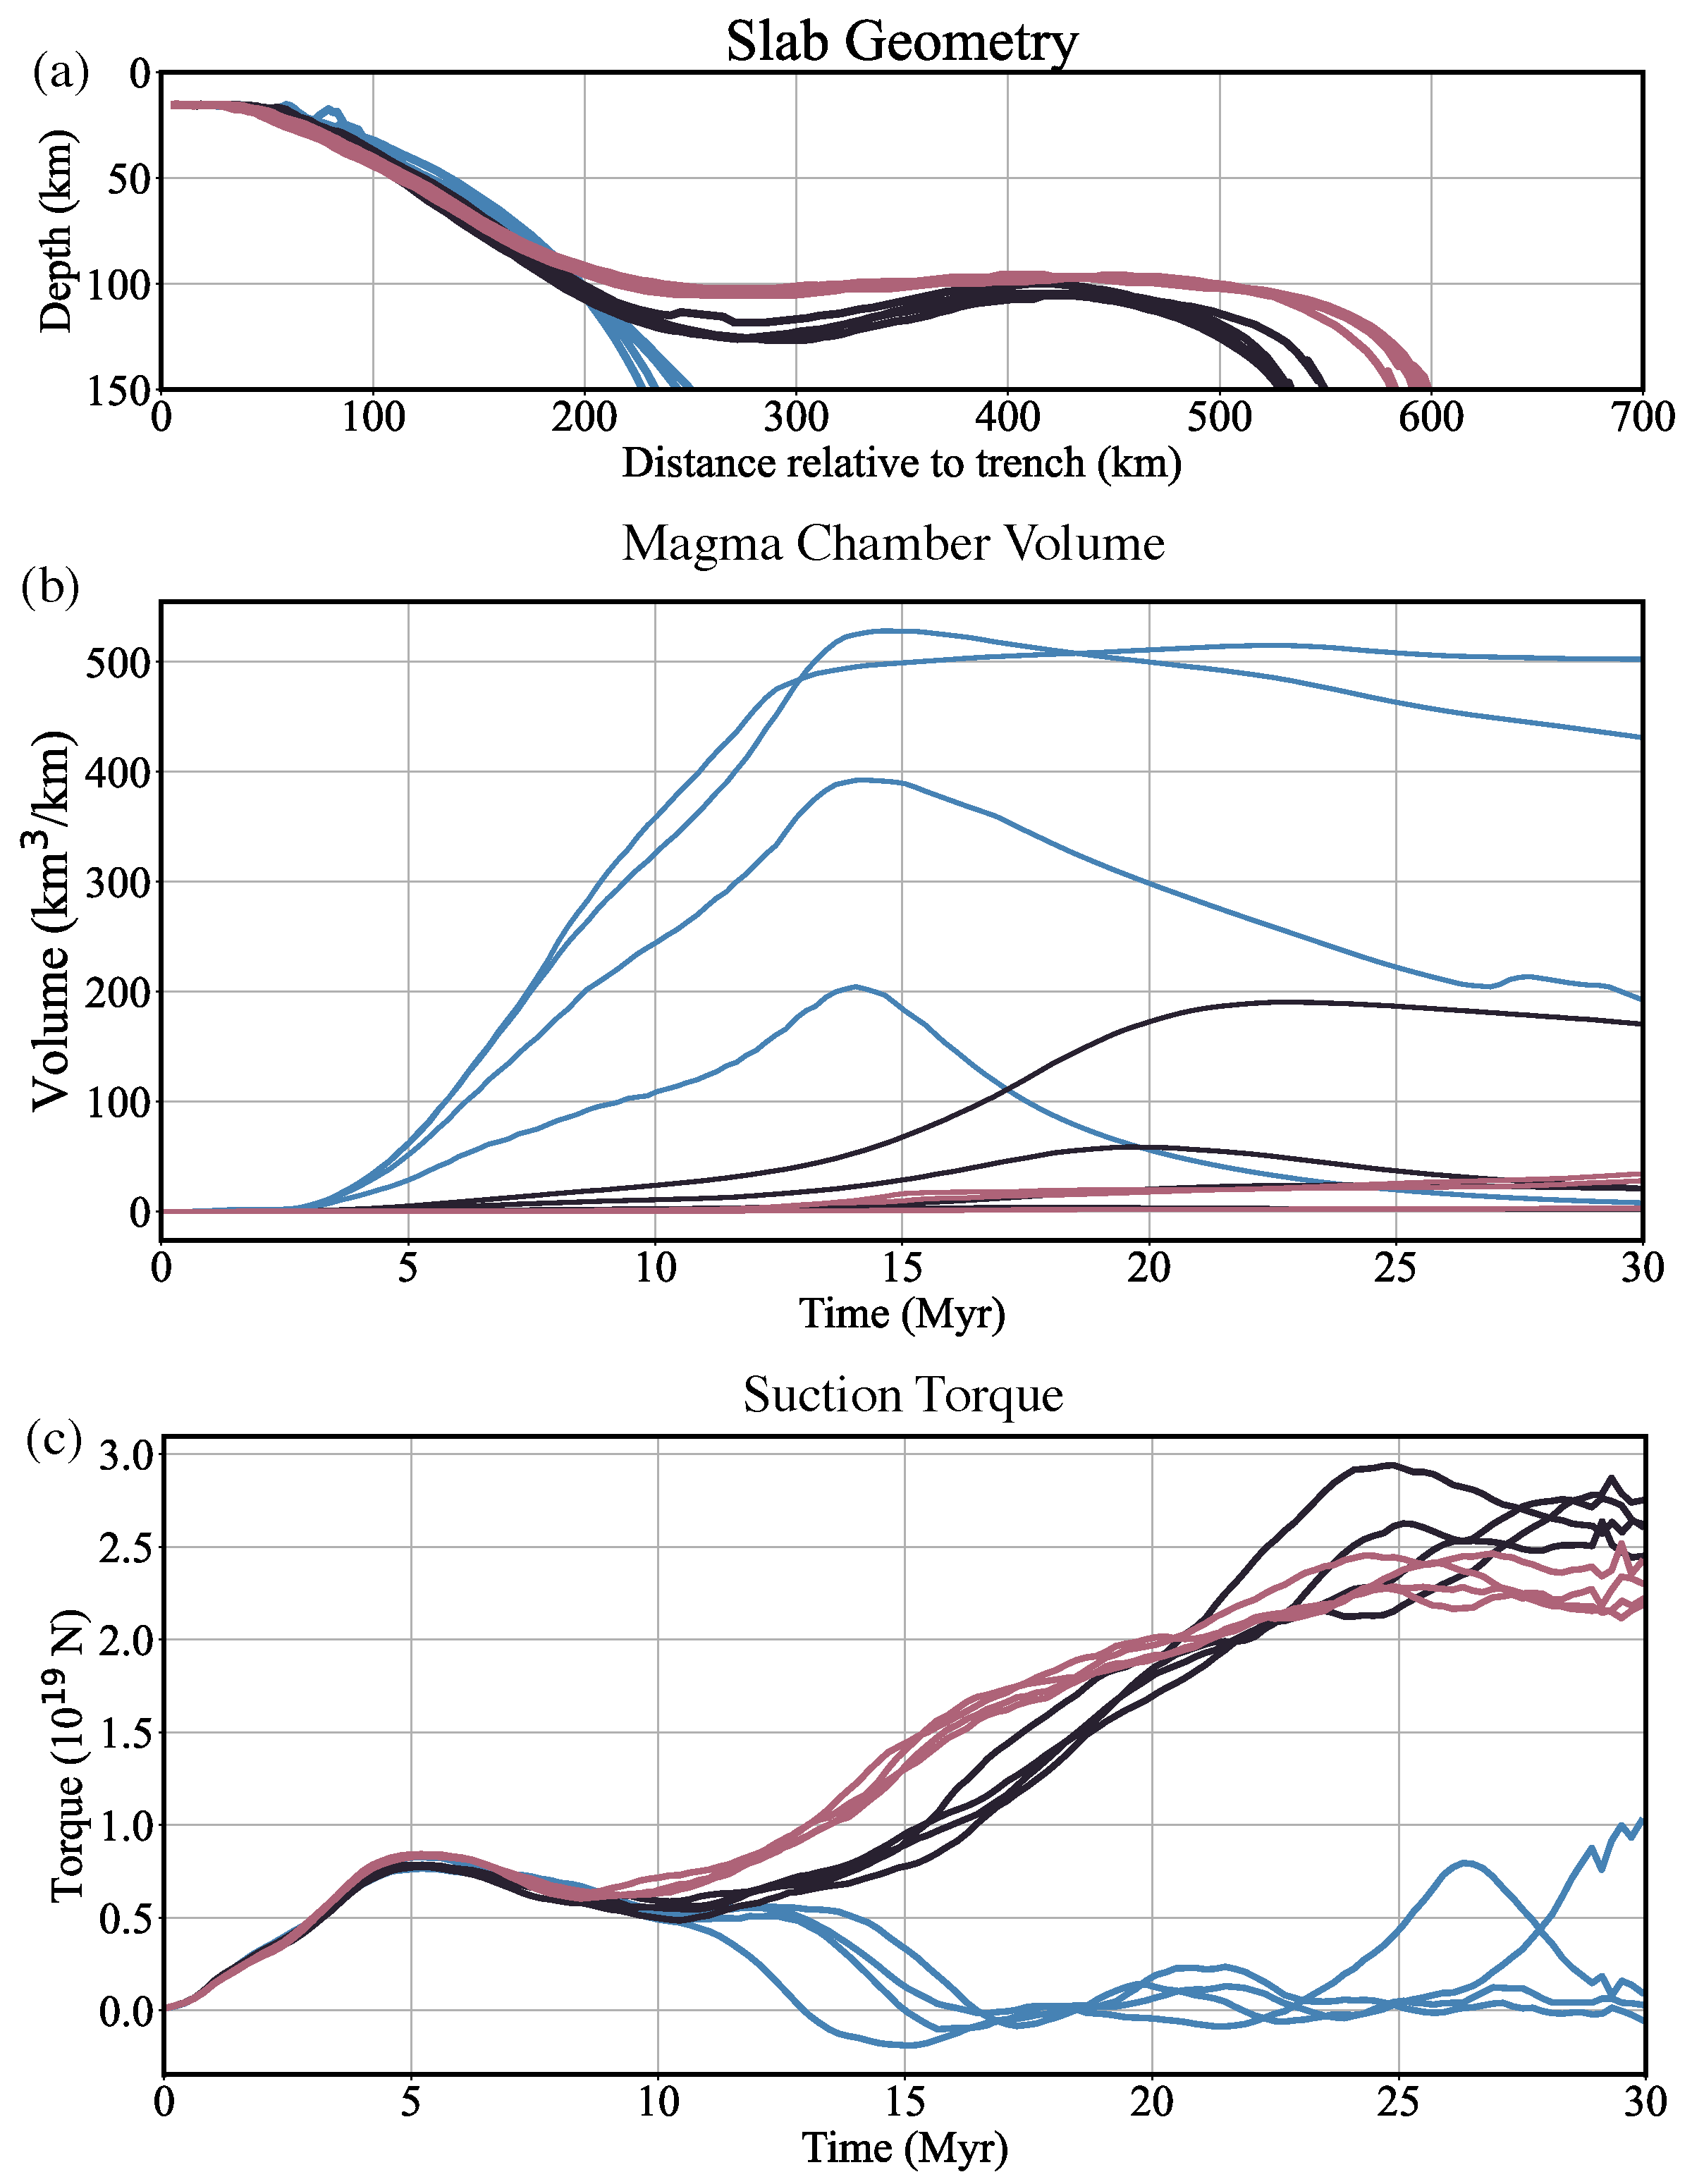
\includegraphics[width=6in]{magma_area_compare.pdf}
    \caption[]{}
    \label{fig::magma_area_compare_Nazca}
\end{figure*}

這些模型中,岩漿產生速率$P=1e13$時的岩漿庫體積在5個百萬年後開始急劇增加,一但模型中的岩漿庫在15個百萬年之前體積超過200$km^3/km$,則模型變會成為一正常隱沒帶,而非平坦隱沒。

\section{本研究的不足之處}
在智利參考模型中,平坦隱沒的特徵在隱沒早期便出現,亦即該模型並不是從一正常傾角的隱沒帶漸變成平坦隱沒。
納茲卡隱沒帶的已存在超過150個百萬年,諸多研究表明,平坦隱沒的發育時間約從10 Myr前後開始,在更早期的隱沒板塊應為正常傾角。
近年來的研究支持平坦隱沒可能與隱沒板塊與660不連續面的交互作用有關,然而本研究智利參考模型僅300公里,無法參與這部分的討論。

本研究的墨西哥參考模型在模型時間前10個百萬年屬於正常的隱沒傾角。

本研究使用的數值模型為二維模型,僅能模擬與海溝垂直的構造變化,無法描述隱沒板塊的側向變化。

本研究的墨西哥模型平坦段長度隨時間逐漸變長,只包含該區域平坦隱沒演化的前半段,
在

本研究目前只能提供影響動水壓力的因素,但無法量化其影響動水壓力的量值。